% ===== UNIT 29: VeRi-Wild: setup, table, figure (5.10 part 1) =====
% Status: AI-DRAFT  (change to REWRITTEN / REVIEWED when done; see CHECKLIST.md)
% Rules: style rewrite only. Keep every \cite, \ref, \label, number, equation and table value as is. Change the wording, not the content.
\subsection{Cross-dataset generalisation on VeRi-Wild}
\label{sec:veriwild}
A central question for any VeRi-776 result is whether it reflects transferable
re-identification ability or dataset-specific tuning. To probe this, we
evaluate our VeRi-776-trained checkpoints zero-shot on
VeRi-Wild~\cite{lou2019veriwild} (416{,}314 images, 40{,}671 identities, 174
cameras), applying the identical feature extraction and post-processing with
no fine-tuning. VeRi-Wild's 174 cameras do not correspond to VeRi-776's
twenty, so no remapping is attempted: the Stream~1 camera side-information
embedding is fixed to a single constant index for all images (one shared camera
token, so the SIE offset is identical everywhere and cancels in relative
comparisons); disabling camera/view embeddings is standard practice in
cross-dataset ReID evaluation~\cite{benmabrouk2026genlimits}, and measured
in-domain on VeRi-776 this substitution costs 2.6\,pp raw mAP
(82.30\%$\rightarrow$79.75\%), so it cannot explain the transfer gap reported
below. As a further control, the transfer evaluation code path was re-run
unchanged on VeRi-776, where it reproduces the in-domain trajectory (raw,
$+$AQE, both streams) to within 0.1\,pp. We report all three official test
protocols (3{,}000\,/\,5{,}000\,/\,10{,}000 identities: equally many queries
against 38{,}861\,/\,64{,}389\,/\,128{,}517 gallery images respectively, from
the official split lists), excluding same-camera--same-identity matches per the
official protocol.

\begin{table*}[!t]
  \centering
  \caption{Zero-shot VeRi-776$\rightarrow$VeRi-Wild transfer across all three
  official test protocols, in context. Top block: our VeRi-776-trained streams,
  using no VeRi-Wild data of any kind (identical extraction and post-processing
  to VeRi-776). Middle block: published VehicleID$\rightarrow$VeRi-Wild
  transfer results as reported in~\cite{zheng2020vapc}; the UDA methods
  additionally adapt on unlabelled VeRi-Wild images, and VehicleID
  provides over twenty times more training identities than VeRi-776. Bottom
  block (different regime, reference only): supervised training on VeRi-Wild's
  own training set. Cells are mAP\,/\,Rank-1 in \%; our best zero-shot
  configuration in \textbf{bold}. Re-ranked transfer rows are measured at the
  3{,}000 protocol only; note re-ranking reduces transfer accuracy.
  Paired-bootstrap 95\% CIs on our mAPs are within $\pm 1.0$\,pp at every
  scale}
  \label{tab:veriwild}
  \small
  \begin{tabular}{L{4.4cm}L{2.0cm}L{2.0cm}C{2.0cm}C{2.0cm}C{2.0cm}}
    \toprule
    & & VeRi-Wild & \multicolumn{3}{c}{Test protocol (mAP\,/\,R1)} \\
    \cmidrule(lr){4-6}
    Method & Source & data used & 3{,}000 & 5{,}000 & 10{,}000 \\
    \midrule
    ViT-B raw (ours)             & VeRi-776 & none & 31.7\,/\,58.7 & 26.7\,/\,52.3 & 20.9\,/\,43.9 \\
    ViT-B $+$AQE (ours)          & VeRi-776 & none & \textbf{35.9}\,/\,\textbf{60.3} & \textbf{30.5}\,/\,\textbf{53.1} & \textbf{23.8}\,/\,\textbf{44.4} \\
    ViT-B $+$AQE$+$rerank (ours) & VeRi-776 & none & 34.8\,/\,57.0 & --- & --- \\
    CLIP-SENet raw (ours)        & VeRi-776 & none & 20.2\,/\,40.6 & 16.8\,/\,35.9 & 12.2\,/\,27.9 \\
    CLIP-SENet $+$AQE (ours)     & VeRi-776 & none & 22.9\,/\,37.1 & 18.9\,/\,32.3 & 13.7\,/\,25.4 \\
    Fusion raw (ours)            & VeRi-776 & none & 28.7\,/\,54.2 & 24.2\,/\,47.6 & 18.5\,/\,38.6 \\
    Fusion $+$AQE (ours)         & VeRi-776 & none & 33.6\,/\,57.3 & 28.1\,/\,50.0 & 21.4\,/\,41.5 \\
    Fusion $+$AQE$+$rerank (ours)& VeRi-776 & none & 30.9\,/\,49.3 & --- & --- \\
    \midrule
    SPGAN~\cite{deng2018spgan}          & VehicleID & unlabelled & 24.1\,/\,59.1 & 21.6\,/\,55.0 & 17.5\,/\,47.4 \\
    UDAP~\cite{song2020udap}            & VehicleID & unlabelled & 30.0\,/\,68.4 & 26.2\,/\,62.5 & 20.8\,/\,53.7 \\
    ECN~\cite{zhong2019ecn}             & VehicleID & unlabelled & 34.7\,/\,73.4 & 30.6\,/\,68.6 & 24.7\,/\,61.0 \\
    VAPC (direct)~\cite{zheng2020vapc}  & VehicleID & none       & 37.7\,/\,74.0 & 33.1\,/\,68.1 & 26.3\,/\,60.2 \\
    VAPC (adapted)~\cite{zheng2020vapc} & VehicleID & unlabelled & 39.7\,/\,75.3 & 34.5\,/\,69.0 & 27.4\,/\,61.0 \\
    \midrule
    FDA-Net~\cite{lou2019veriwild}      & VeRi-Wild & labelled & 35.1\,/\,--- & 29.8\,/\,--- & 22.8\,/\,--- \\
    CLIP-SENet~\cite{lu2025clipsenet}   & VeRi-Wild & labelled & 89.1\,/\,97.9 & 85.2\,/\,97.0 & 79.5\,/\,95.4 \\
    \bottomrule
  \end{tabular}
\end{table*}

\begin{figure*}[!t]
  \centering
  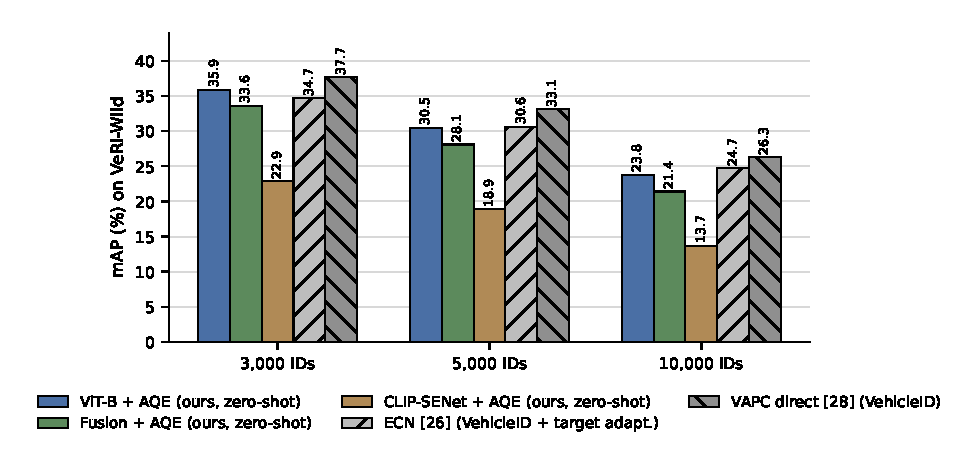
\includegraphics[width=0.86\textwidth]{Fig10}
  \caption{Zero-shot VeRi-776$\rightarrow$VeRi-Wild transfer across the three
  official protocols, compared with published VehicleID-sourced transfer
  methods. Our streams use no VeRi-Wild data of any kind, whereas ECN
  additionally adapts on unlabelled target images and both comparison methods
  draw on a source with over twenty times more identities. The ViT-B stream
  transfers competitively at every scale; the fusion falls below it everywhere}
  \label{fig:transfer}
\end{figure*}
